\begin{figure}[tp]
\centering
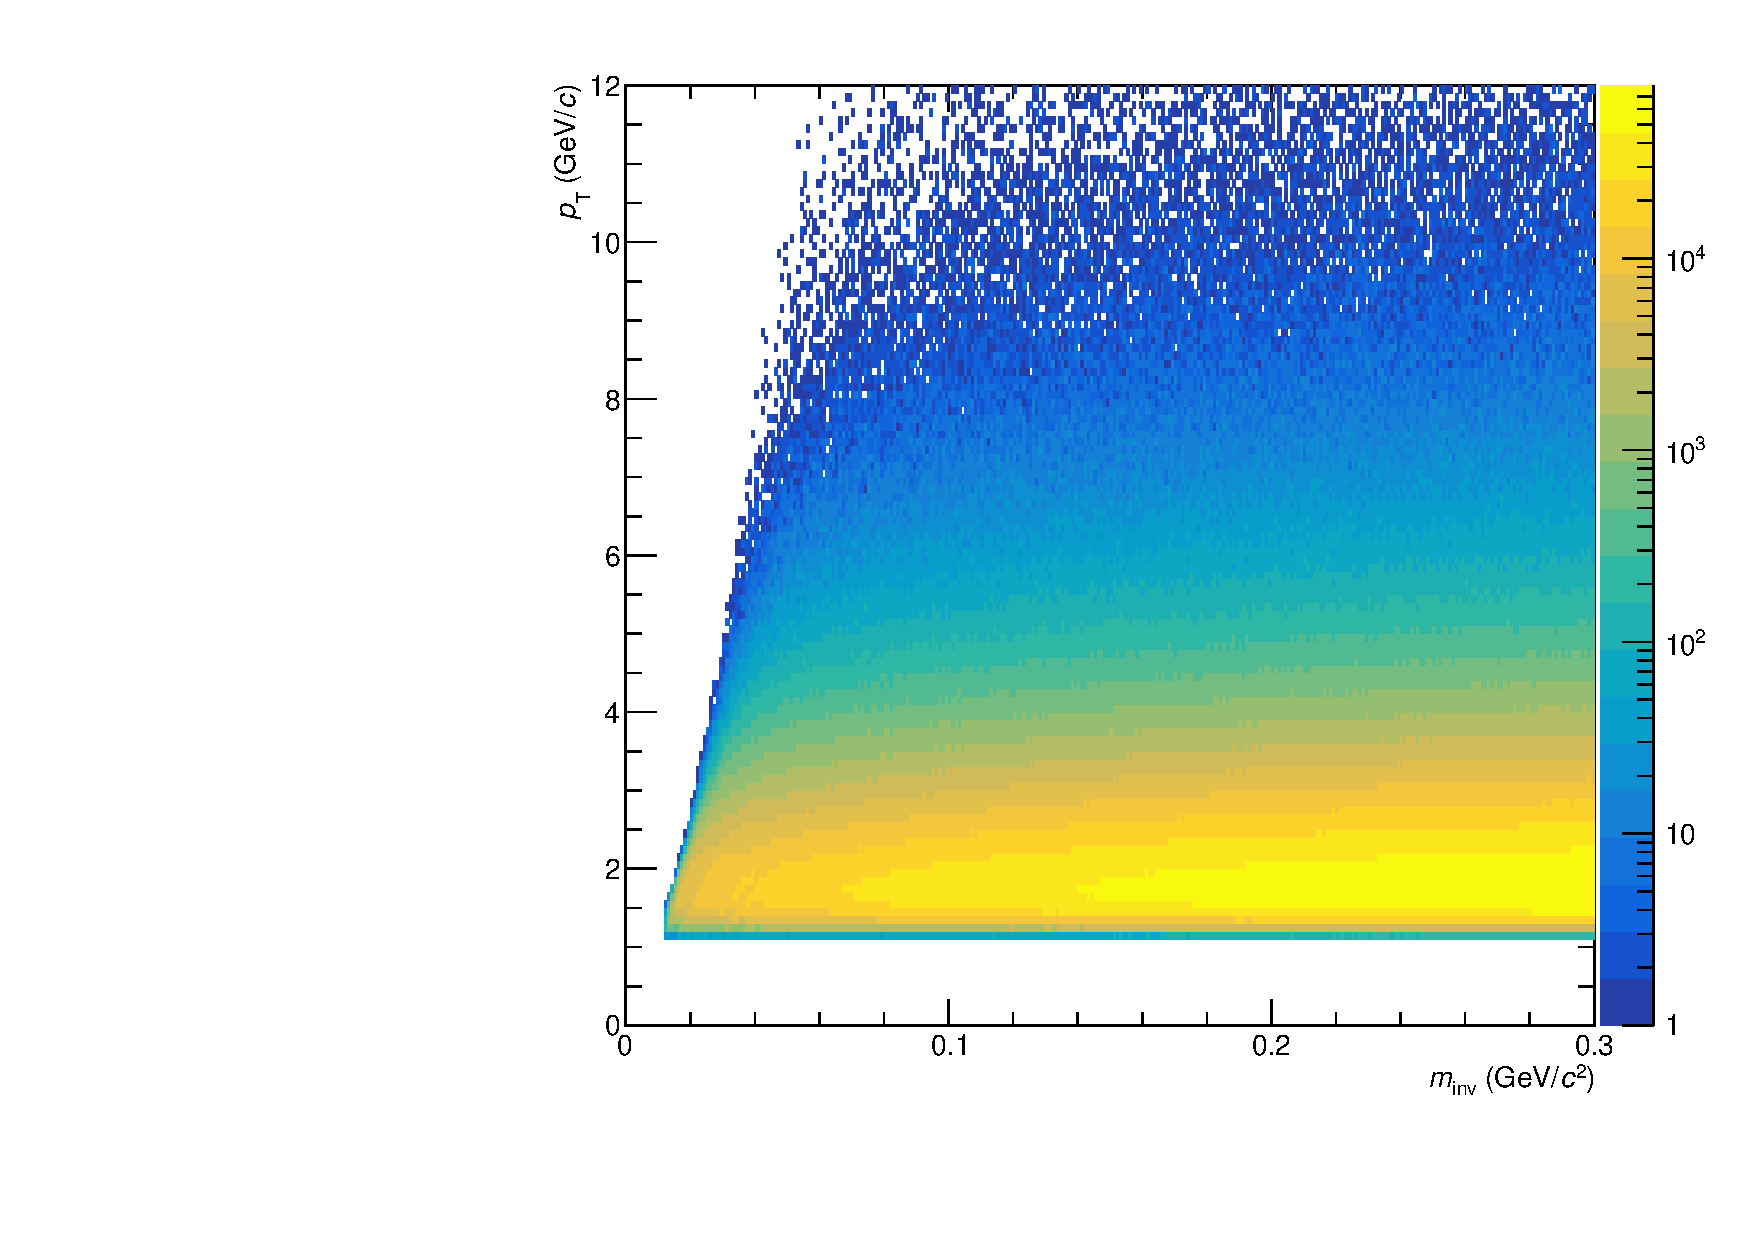
\includegraphics[width=.7\linewidth]{hInvMass_pT_Bkg.pdf}
\caption{$p_\text{T}$ und $m_\text{inv}$ als Funktion von der Anzahl von rekombinierten  Cluster-Paaren aus unterschiedlichen Kollision.}
\label{figInvMassPt_b}
\end{figure}
Durch das paarweise kombinieren aller Photonenkandidaten, wie es in Abschnitt \ref{s3s2} gezeigt wurde, besteht ein gro{\ss}er Anteil der rekonstruierten Datenpunkte aus unkorreliert Paaren.
Das hei{\ss}t, dass die beiden Photonenkandidaten nicht \"uber einen Zerfall zusammenh{"a}ngen.
Um den unkorrelierten Untergrund abzusch\"atzen werden Photonenkandidaten aus unterschiedlichen \textit{Events} mit Hilfe der sogenannten \textit{mixed event method} miteinander kombiniert.
Abbildung \ref{figInvMassPt_b} zeigt eine solche Verteilung, bei der Photonenkandidaten aus unterschiedlichen Kollisionen miteinander kombiniert wurden.
Eine H\"aufung der Datenpunkte um eine bestimmte invariante Masse gibt es, wie zu erwarten, nicht.
Die linke Flanke aufgrund der \textit{\"Offnungwinkel-cuts} hingegen bleibt bestehen.
%\begin{figure}[tp]
%\centering
%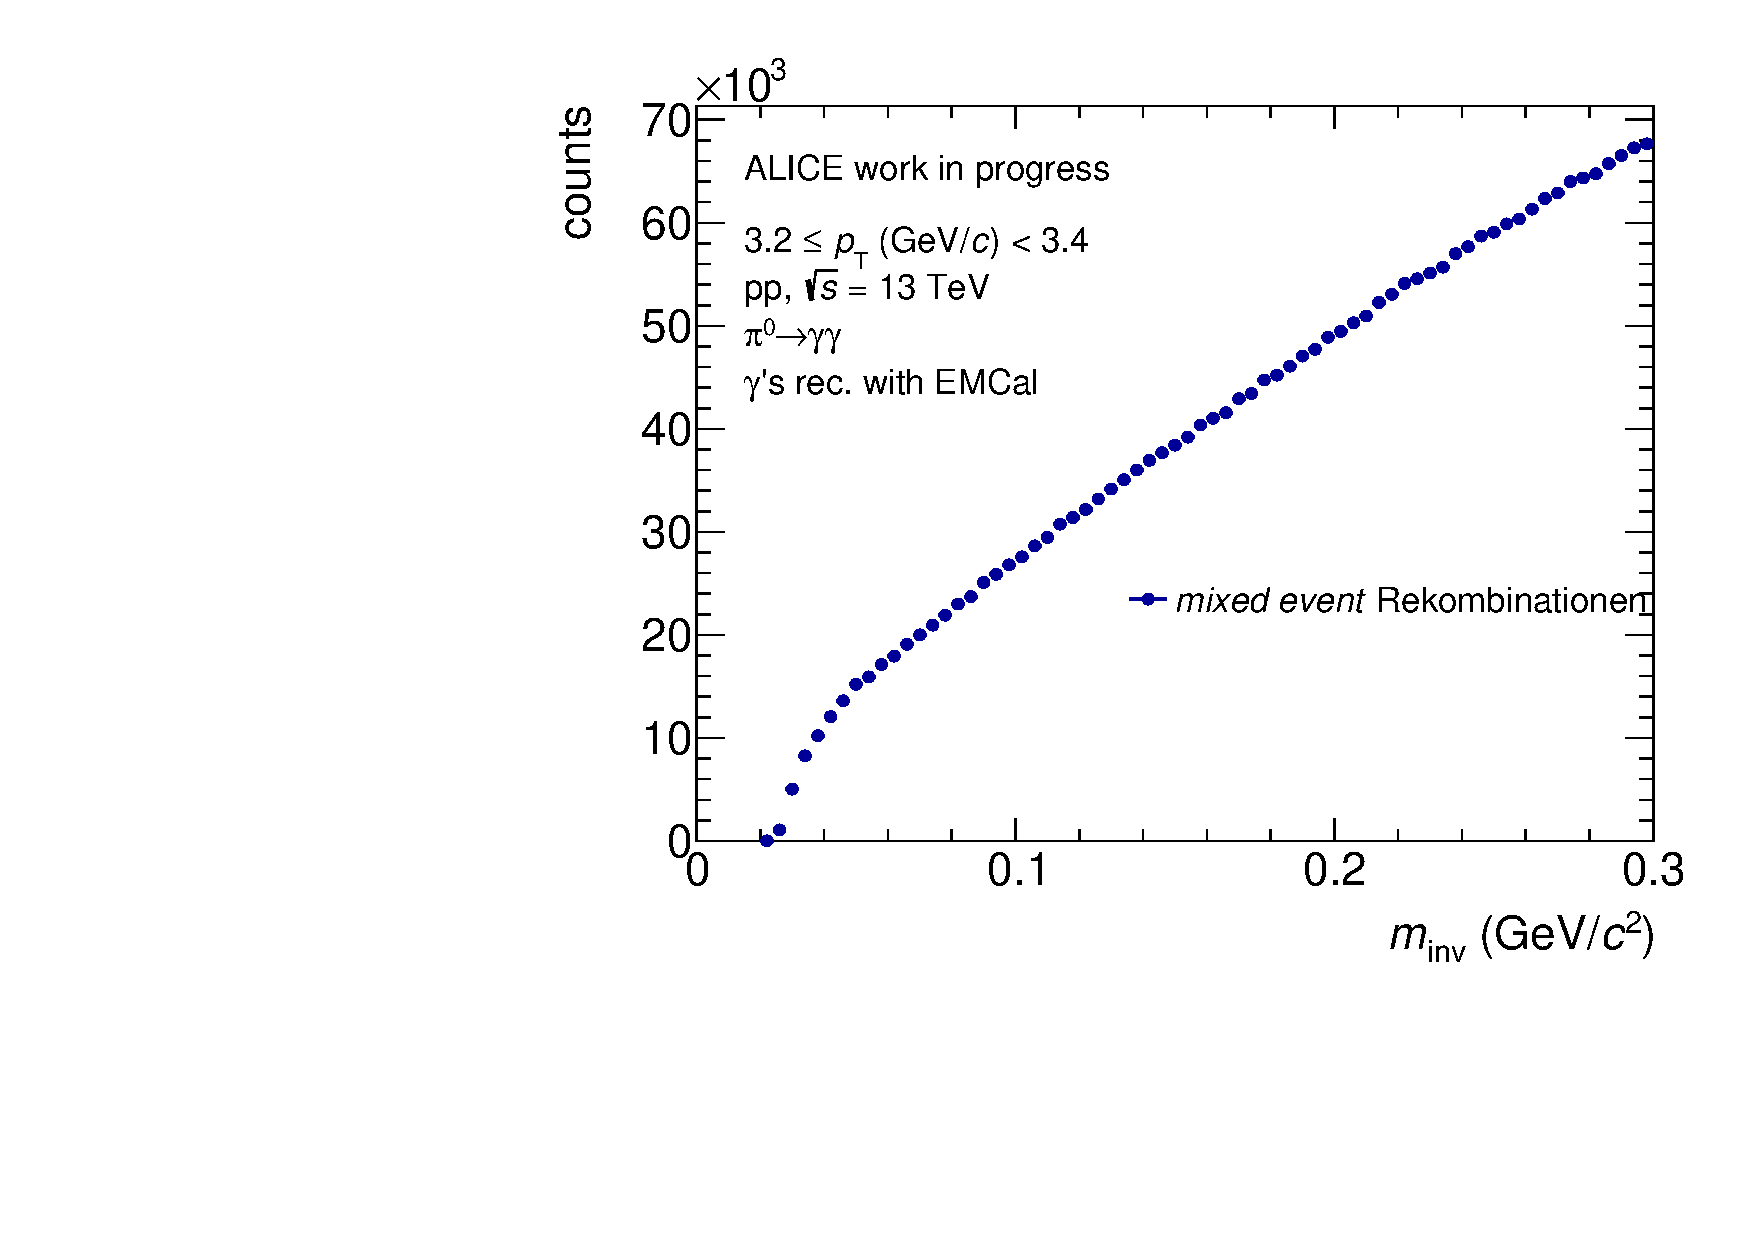
\includegraphics[width=.75\linewidth]{hUncorrBkg.pdf}
%\caption{Kombinationen von Photonenkandidaten aus unterschiedlichen Kollisionen, die keine Korrelationen zueinander haben, weshalb auch kein Peak im Bereich der $\pi^{0}$-Masse zu sehen ist. Dies dient als Grundlage zur Bestimmung des unkorrelierten Untergrunds.}
%\label{figUncorrBkg}
%\end{figure}
\newline
%Auch die \textit{mixed event} Verteilung wird in den gleichen $p_{\rm{T}}$-Intervallen integriert betrachtet wie zuvor die \textit{same event} Verteilung.
%Abbildung \ref{figUncorrBkg} zeigt die invariante Massenverteilung f\"ur das $p_{\text{T}}$-Intervall $(3,2 - 3,4) (\text{GeV/}c)$.
%Diese Verteilung weist keinen Peak auf und hat eine gr{\"o}{\ss}ere Anzahl Eintr{\"a}ge, als die Verteilung aus der \textit{same event method}.
Aufgrund der gr{\"o}{\ss}eren Anzahl Eintr{\"a}ge, da es in der \textit{mixed event method} mehr Kombinationsm\"oglichkeiten gibt als in der \textit{same event method} muss die Verteilung aus der \textit{mixed event method} an die aus der \textit{same event method} skaliert werden.
Die Skalierung erfolgt im rechten Bereich au{\ss}erhalb des $\pi^{0}$-Peaks bei $m_\text{inv} \in \left[0,19;3,0\right] (\text{GeV/}c^{2})$ und es ergibt sich f{\"u}r den Skalierungsfaktor:
\begin{align}
\label{eqBackSkalierung}
\alpha &= \frac{\sum_{i \neq j}\sum_{n}m_{\text{inv}}\left( \gamma^{(n)}_{i},\gamma^{(n)}_{j}\right) }{\sum_{i,j}\sum_{n \neq m}m_{\text{inv}}\left( \gamma^{(n)}_{i},\gamma^{(m)}_{j}\right) }
\end{align}
Die oberen Indize $m$ und $n$ stehen hierbei f{\"u}r ein Event, aus dem ein Photon kommt und die unteren Indize $i$ und $j$ numerieren die Photonen ($\gamma$).
\begin{figure}[tp]
\centering
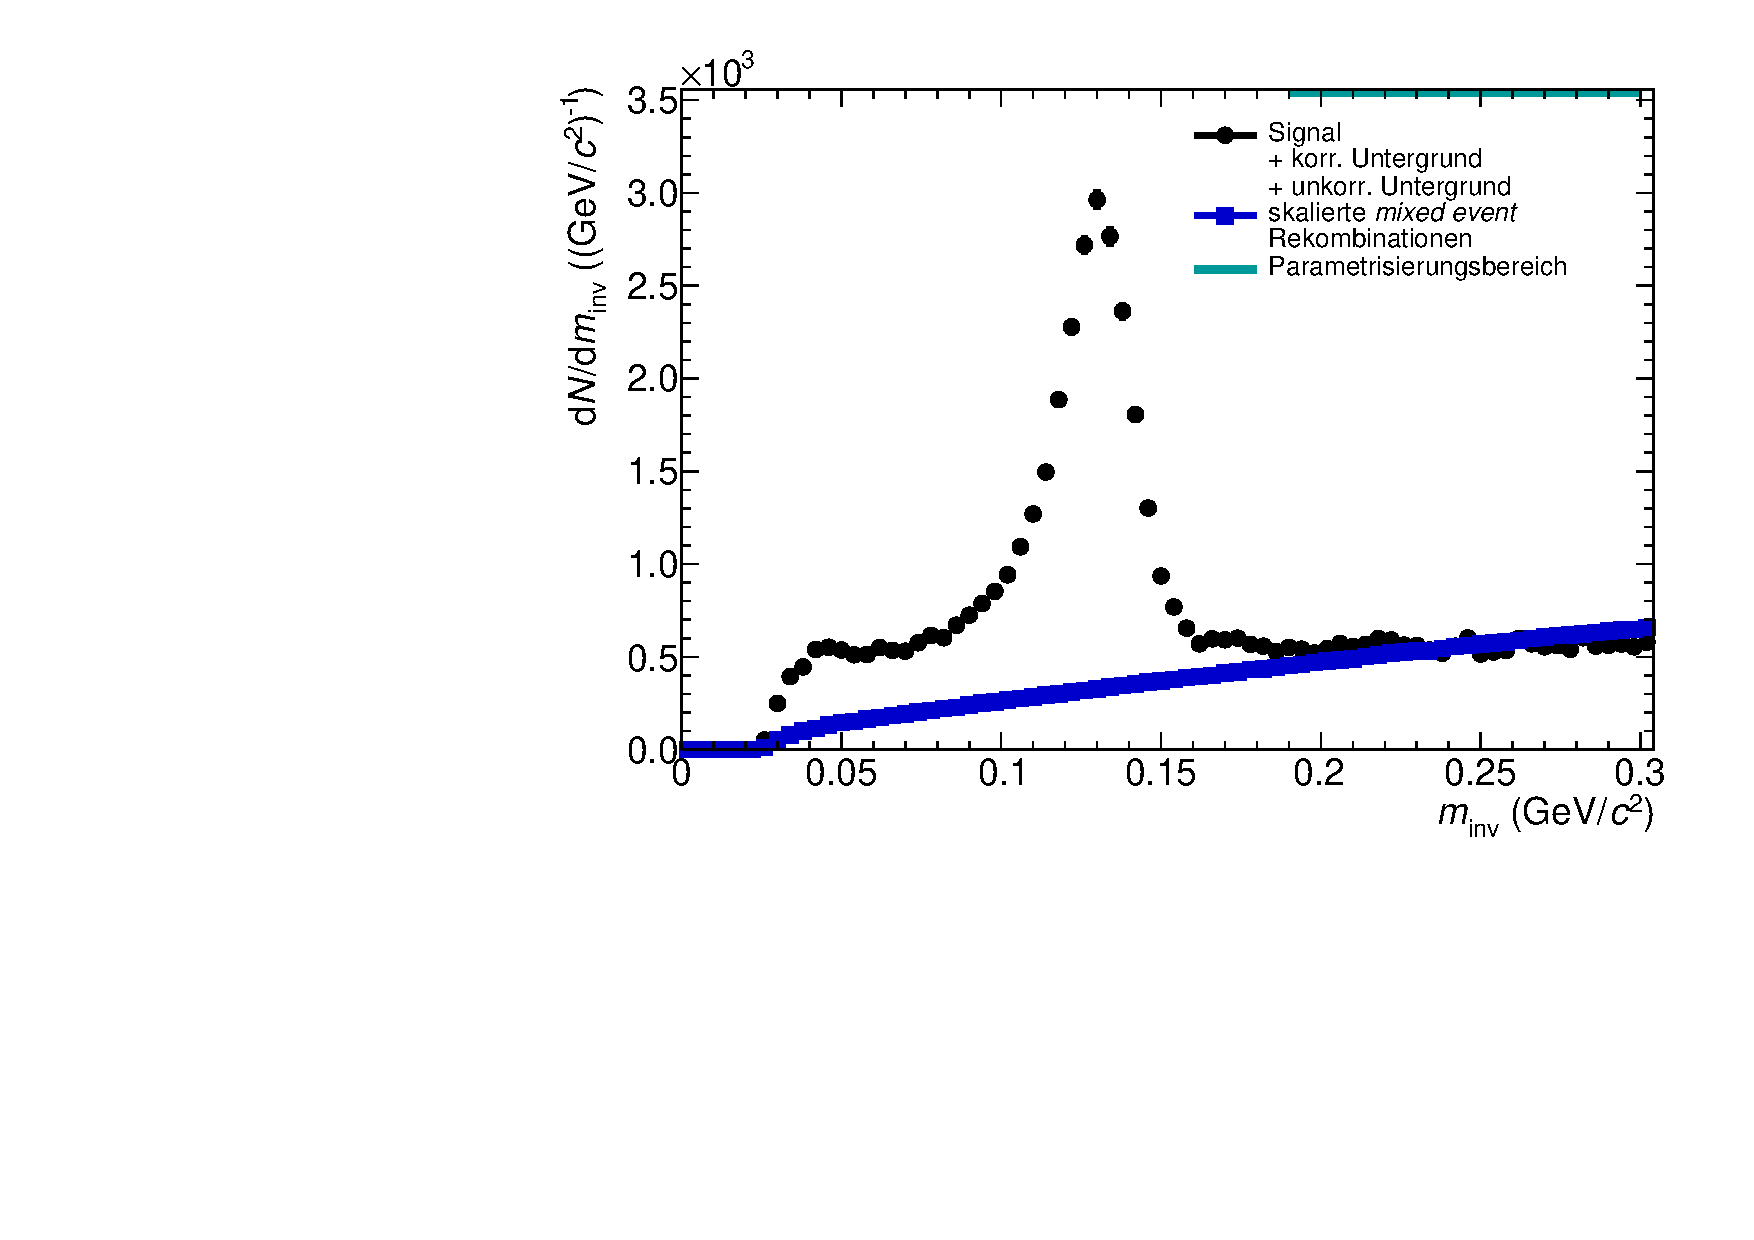
\includegraphics[width=.75\linewidth]{hUncorrBkgNorm.pdf}
\caption{Nach Gleichung \ref{eqBackSkalierung} skalierte {\it mixed event} Rekombinationen aus Abbildung \ref{figUncorrBkg} als Absch{\"a}tzung des unkorrelierten Untergrunds zusammen aufgetragen mit Signal zuz{\"u}glich beiden Untergrundkomponenten wie in Abbildung \ref{figSignalPlusBkg}.}
\label{figUncorrBkgNorm}
\end{figure}
\newline
Das Resultat der Skalierung ist in Abbildung \ref{figUncorrBkgNorm} zu sehen, wo zus{\"a}tzlich noch das Signal eingezeichnet ist, um besser erkennen zu k{\"o}nnen, wie sich der abgesch{\"a}tzte unkorrelierte Untergrund relativ zum gesamten Signal verh{\"a}lt.
Nachdem der unkorrelierte Untergrund abgesch\"azt wurde wird dieser vom Signal subtrahiert.
\begin{figure}[tbp]
\centering
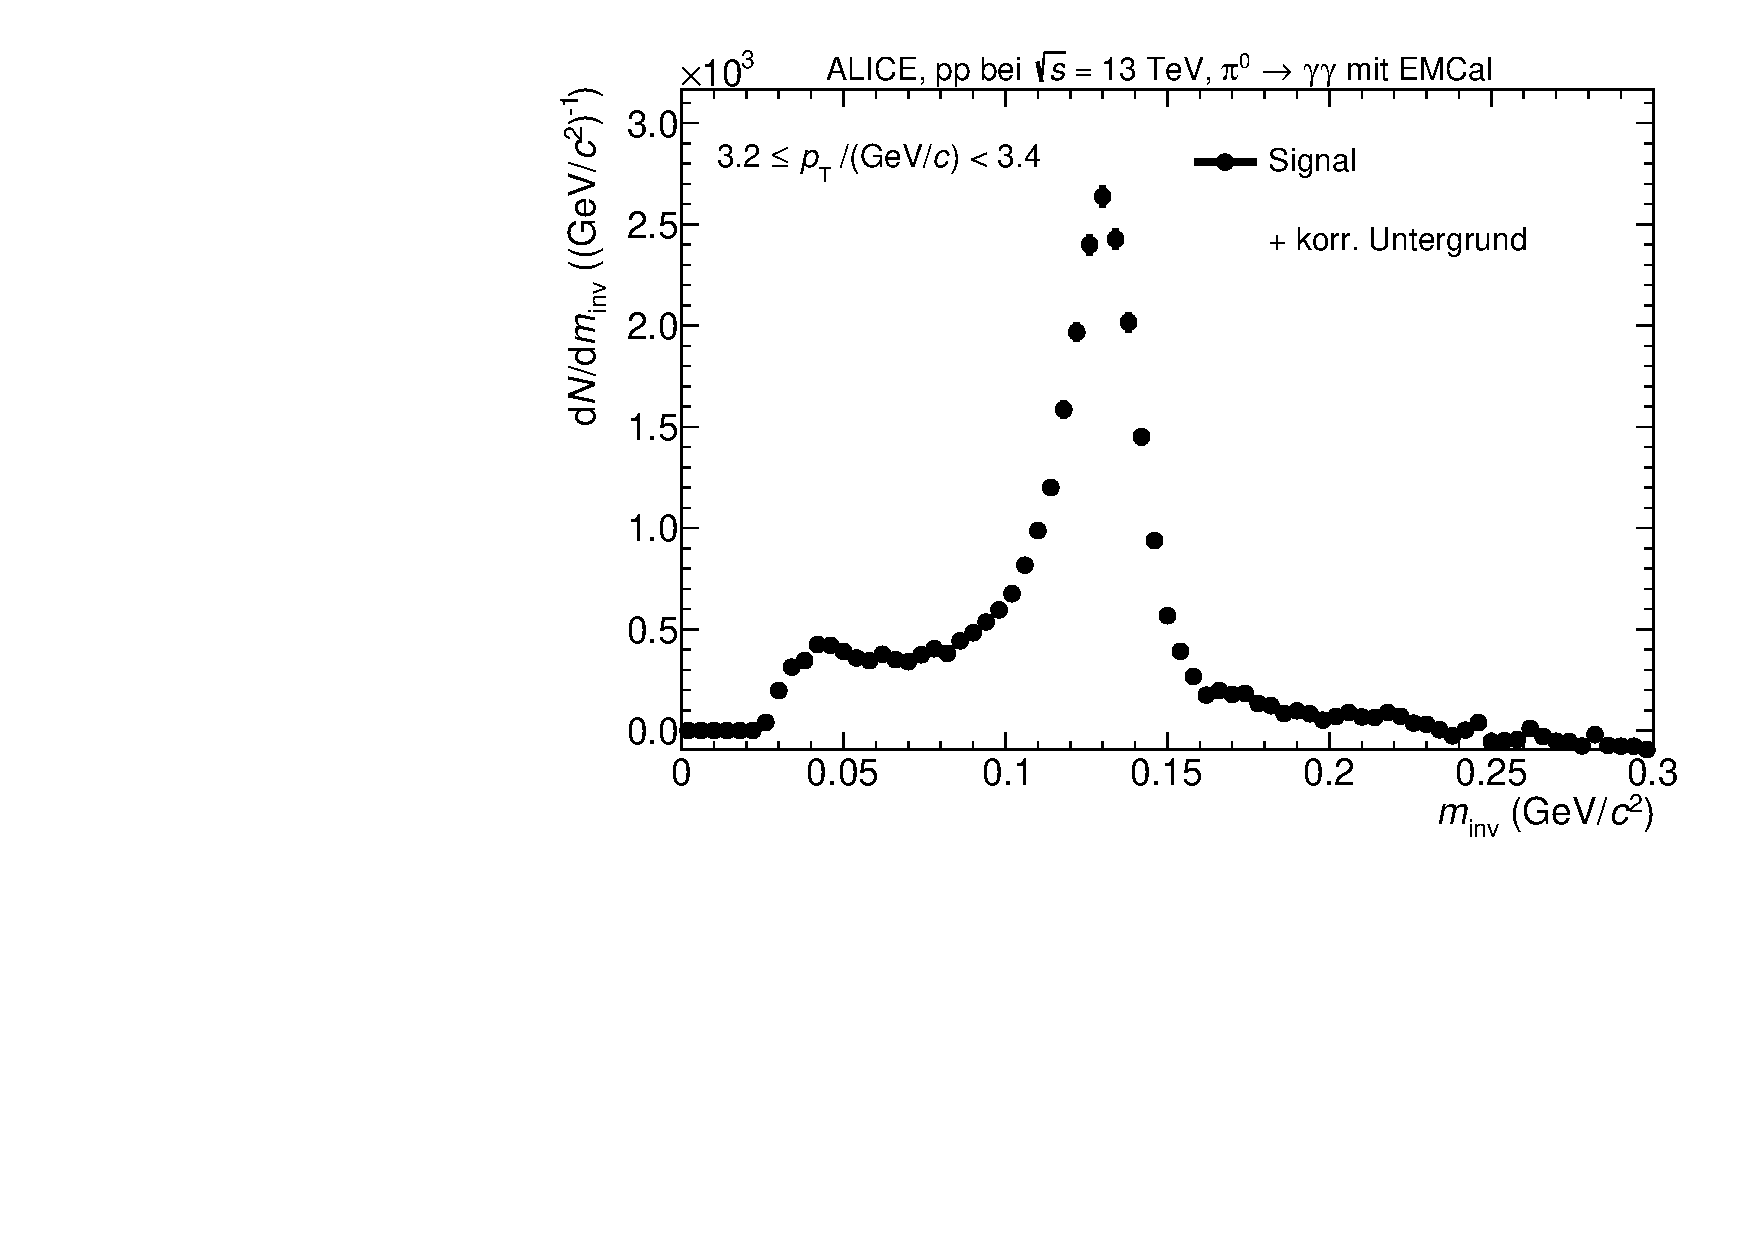
\includegraphics[width=.75\linewidth]{hInvMass_Data.pdf}
\caption{Signal nach Abzug des unkorrelierten Untergrunds.}
\label{figInvMass_Data}
\end{figure}
\newline
Abbildung \ref{figInvMass_Data} zeigt das Ergebnis des Abzugs des unkorrelierten Untergrunds vom Signal.
Da Photonen durch Paarbildung in ein Elektron und ein Positron zerfallen k\"onnen, bestehen einige Photonenkandidaten aus \textit{Clustern} von nur einem der beiden Zerfallsprodukte.
Diese Photonenkandidaten weisen dann eine geringere Energie auf, als das eigentliche Photon besa{\ss}.
Durch Kombinationen mit diesen Photonenkandidaten entstehen Datenpunkte bei einer invarianten Masse, die meistens geringer ist als die Masse von $\pi^{0}$, obwohl beide Photonenkandidaten dem selben $\pi^{0}$ entstammen.
Deshalb wird kleineren invarianten Massen vom Peak ein Teil des Signals erwartet, jedoch auch korrelierter Untergrund.
\newline
Die Bestimmung des korrelierten Untergrunds, ist eine wichtige Aufgabe in der Analyse von neutralen Pionen.
Das Absch\"atzen mit einer linearen Funktion hat sich als g\"angiste Methode zur Bestimmung des korrelierten Untergrunds entwickelt und wird im Folgenden als Standardmethode bezeichnet.
In dieser Arbeit wird der korrelierte Untergr\"und sowie das reine $\pi^{0}$-Signal mit Hilfe von sogenannten \textit{Monte Carlo Templates} bestimmt.
Die Ergebnisse der Analyse mit Hilfe von Monte Carlo Templates, sowie mit der Standardmethode werden miteinander vergleichen, um eine Aussage \"uber den m\"oglichen Nutzen von Analysen mit Hilfe von Monte Carlo Templates treffen zu k\"onnen.
Im folgenden Abschnitt wird sowohl die Standardmethode kurz, als auch die Methode mit Hilfe von Monte Carlo Templates n\"aher erl\"autert.